

\tikzset{every picture/.style={line width=0.75pt}} %set default line width to 0.75pt        

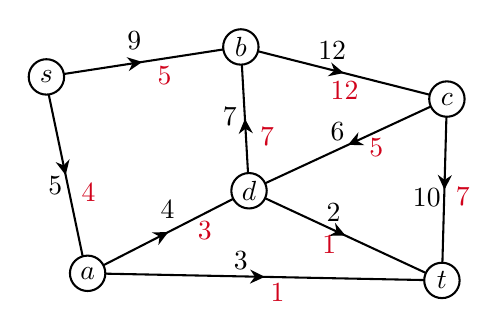
\begin{tikzpicture}[x=0.5pt,y=0.5pt,yscale=-1,xscale=1]
%uncomment if require: \path (0,222); %set diagram left start at 0, and has height of 222

%Straight Lines [id:da3853598268579197] 
\draw    (24.79,46.83) -- (165.31,25.18) ;
\draw [shift={(95.05,36)}, rotate = 531.24] [fill={rgb, 255:red, 0; green, 0; blue, 0 }  ][line width=0.08]  [draw opacity=0] (10.72,-5.15) -- (0,0) -- (10.72,5.15) -- (7.12,0) -- cycle    ;
%Straight Lines [id:da6958538828947681] 
\draw    (24.79,46.83) -- (54.58,188.77) ;
\draw [shift={(39.69,117.8)}, rotate = 258.15] [fill={rgb, 255:red, 0; green, 0; blue, 0 }  ][line width=0.08]  [draw opacity=0] (10.72,-5.15) -- (0,0) -- (10.72,5.15) -- (7.12,0) -- cycle    ;
%Straight Lines [id:da2980592918523626] 
\draw    (55.58,188.77) -- (311.62,193.9) ;
\draw [shift={(183.6,191.34)}, rotate = 181.15] [fill={rgb, 255:red, 0; green, 0; blue, 0 }  ][line width=0.08]  [draw opacity=0] (10.72,-5.15) -- (0,0) -- (10.72,5.15) -- (7.12,0) -- cycle    ;
%Straight Lines [id:da14604600957867897] 
\draw    (172.22,129.11) -- (311.62,193.9) ;
\draw [shift={(241.92,161.5)}, rotate = 204.92000000000002] [fill={rgb, 255:red, 0; green, 0; blue, 0 }  ][line width=0.08]  [draw opacity=0] (10.72,-5.15) -- (0,0) -- (10.72,5.15) -- (7.12,0) -- cycle    ;
%Straight Lines [id:da8640956582518242] 
\draw    (166.31,25.18) -- (172.22,129.11) ;
\draw [shift={(169.27,77.14)}, rotate = 86.75] [fill={rgb, 255:red, 0; green, 0; blue, 0 }  ][line width=0.08]  [draw opacity=0] (10.72,-5.15) -- (0,0) -- (10.72,5.15) -- (7.12,0) -- cycle    ;
%Straight Lines [id:da285469110869773] 
\draw    (166.31,25.18) -- (315.22,62.84) ;
\draw [shift={(240.76,44.01)}, rotate = 194.2] [fill={rgb, 255:red, 0; green, 0; blue, 0 }  ][line width=0.08]  [draw opacity=0] (10.72,-5.15) -- (0,0) -- (10.72,5.15) -- (7.12,0) -- cycle    ;
%Straight Lines [id:da8162300663234149] 
\draw    (315.22,62.84) -- (311.62,193.9) ;
\draw [shift={(313.42,128.37)}, rotate = 271.57] [fill={rgb, 255:red, 0; green, 0; blue, 0 }  ][line width=0.08]  [draw opacity=0] (10.72,-5.15) -- (0,0) -- (10.72,5.15) -- (7.12,0) -- cycle    ;
%Straight Lines [id:da5085854502811855] 
\draw    (315.22,62.84) -- (172.22,129.11) ;
\draw [shift={(243.72,95.98)}, rotate = 335.13] [fill={rgb, 255:red, 0; green, 0; blue, 0 }  ][line width=0.08]  [draw opacity=0] (10.72,-5.15) -- (0,0) -- (10.72,5.15) -- (7.12,0) -- cycle    ;
%Straight Lines [id:da4064365628912957] 
\draw    (172.22,129.11) -- (55.58,188.77) ;
\draw [shift={(113.9,158.94)}, rotate = 152.91] [fill={rgb, 255:red, 0; green, 0; blue, 0 }  ][line width=0.08]  [draw opacity=0] (10.72,-5.15) -- (0,0) -- (10.72,5.15) -- (7.12,0) -- cycle    ;
%Shape: Ellipse [id:dp651117123053256] 
\draw  [fill={rgb, 255:red, 255; green, 255; blue, 255 }  ,fill opacity=1 ] (13,46.83) .. controls (13,39.77) and (18.73,34.04) .. (25.79,34.04) .. controls (32.86,34.04) and (38.58,39.77) .. (38.58,46.83) .. controls (38.58,53.9) and (32.86,59.62) .. (25.79,59.62) .. controls (18.73,59.62) and (13,53.9) .. (13,46.83) -- cycle ;
%Shape: Ellipse [id:dp7399561756845123] 
\draw  [fill={rgb, 255:red, 255; green, 255; blue, 255 }  ,fill opacity=1 ] (153.52,25.18) .. controls (153.52,18.11) and (159.25,12.39) .. (166.31,12.39) .. controls (173.38,12.39) and (179.1,18.11) .. (179.1,25.18) .. controls (179.1,32.24) and (173.38,37.97) .. (166.31,37.97) .. controls (159.25,37.97) and (153.52,32.24) .. (153.52,25.18) -- cycle ;
%Shape: Ellipse [id:dp8268258265249401] 
\draw  [fill={rgb, 255:red, 255; green, 255; blue, 255 }  ,fill opacity=1 ] (302.43,62.84) .. controls (302.43,55.78) and (308.15,50.05) .. (315.22,50.05) .. controls (322.28,50.05) and (328.01,55.78) .. (328.01,62.84) .. controls (328.01,69.9) and (322.28,75.63) .. (315.22,75.63) .. controls (308.15,75.63) and (302.43,69.9) .. (302.43,62.84) -- cycle ;
%Shape: Ellipse [id:dp5421818862330341] 
\draw  [fill={rgb, 255:red, 255; green, 255; blue, 255 }  ,fill opacity=1 ] (159.43,129.11) .. controls (159.43,122.05) and (165.15,116.32) .. (172.22,116.32) .. controls (179.28,116.32) and (185.01,122.05) .. (185.01,129.11) .. controls (185.01,136.18) and (179.28,141.9) .. (172.22,141.9) .. controls (165.15,141.9) and (159.43,136.18) .. (159.43,129.11) -- cycle ;
%Shape: Ellipse [id:dp45600813719389455] 
\draw  [fill={rgb, 255:red, 255; green, 255; blue, 255 }  ,fill opacity=1 ] (42.79,188.77) .. controls (42.79,181.71) and (48.52,175.98) .. (55.58,175.98) .. controls (62.64,175.98) and (68.37,181.71) .. (68.37,188.77) .. controls (68.37,195.84) and (62.64,201.56) .. (55.58,201.56) .. controls (48.52,201.56) and (42.79,195.84) .. (42.79,188.77) -- cycle ;
%Shape: Ellipse [id:dp031187496945339066] 
\draw  [fill={rgb, 255:red, 255; green, 255; blue, 255 }  ,fill opacity=1 ] (298.83,193.9) .. controls (298.83,186.83) and (304.56,181.11) .. (311.62,181.11) .. controls (318.69,181.11) and (324.41,186.83) .. (324.41,193.9) .. controls (324.41,200.96) and (318.69,206.69) .. (311.62,206.69) .. controls (304.56,206.69) and (298.83,200.96) .. (298.83,193.9) -- cycle ;

% Text Node
\draw (25.79,46.83) node   [align=left] {$\displaystyle s$};
% Text Node
\draw (166.31,25.18) node   [align=left] {$\displaystyle b$};
% Text Node
\draw (315.22,62.84) node   [align=left] {$\displaystyle c$};
% Text Node
\draw (172.22,129.11) node   [align=left] {$\displaystyle d$};
% Text Node
\draw (55.58,188.77) node   [align=left] {$\displaystyle a$};
% Text Node
\draw (311.62,193.9) node   [align=left] {$\displaystyle t$};
% Text Node
\draw (229,48) node [anchor=north west][inner sep=0.75pt]   [align=left] {$\displaystyle \textcolor[rgb]{0.82,0.01,0.11}{12}$};
% Text Node
\draw (25,117) node [anchor=north west][inner sep=0.75pt]   [align=left] {$\displaystyle 5$};
% Text Node
\draw (106,134) node [anchor=north west][inner sep=0.75pt]   [align=left] {$\displaystyle 4$};
% Text Node
\draw (185.6,194.34) node [anchor=north west][inner sep=0.75pt]   [align=left] {$\displaystyle \textcolor[rgb]{0.82,0.01,0.11}{1}$};
% Text Node
\draw (82,12) node [anchor=north west][inner sep=0.75pt]   [align=left] {$\displaystyle 9$};
% Text Node
\draw (229,78) node [anchor=north west][inner sep=0.75pt]   [align=left] {$\displaystyle 6$};
% Text Node
\draw (151,67) node [anchor=north west][inner sep=0.75pt]   [align=left] {$\displaystyle 7$};
% Text Node
\draw (226,136) node [anchor=north west][inner sep=0.75pt]   [align=left] {$\displaystyle 2$};
% Text Node
\draw (319.42,124.37) node [anchor=north west][inner sep=0.75pt]   [align=left] {$\displaystyle \textcolor[rgb]{0.82,0.01,0.11}{7}$};
% Text Node
\draw (133,149) node [anchor=north west][inner sep=0.75pt]   [align=left] {$\displaystyle \textcolor[rgb]{0.82,0.01,0.11}{3}$};
% Text Node
\draw (223,159) node [anchor=north west][inner sep=0.75pt]   [align=left] {$\displaystyle \textcolor[rgb]{0.82,0.01,0.11}{1}$};
% Text Node
\draw (257,89) node [anchor=north west][inner sep=0.75pt]   [align=left] {$\displaystyle \textcolor[rgb]{0.82,0.01,0.11}{5}$};
% Text Node
\draw (178,81) node [anchor=north west][inner sep=0.75pt]   [align=left] {$\displaystyle \textcolor[rgb]{0.82,0.01,0.11}{7}$};
% Text Node
\draw (288.42,125.37) node [anchor=north west][inner sep=0.75pt]   [align=left] {$\displaystyle 10$};
% Text Node
\draw (220,19) node [anchor=north west][inner sep=0.75pt]   [align=left] {$\displaystyle 12$};
% Text Node
\draw (49,122) node [anchor=north west][inner sep=0.75pt]   [align=left] {$\displaystyle \textcolor[rgb]{0.82,0.01,0.11}{4}$};
% Text Node
\draw (104,37) node [anchor=north west][inner sep=0.75pt]   [align=left] {$\displaystyle \textcolor[rgb]{0.82,0.01,0.11}{5}$};
% Text Node
\draw (159,171) node [anchor=north west][inner sep=0.75pt]   [align=left] {$\displaystyle 3$};


\end{tikzpicture}

